\documentclass[11pt, a4paper]{article}

\usepackage[utf8]{inputenc}
\usepackage{amsmath, amssymb, amsthm}
\usepackage{geometry}
\geometry{left=2.5cm, right=2.5cm, top=3cm, bottom=3cm}
\usepackage{hyperref}
\usepackage{graphicx}
\graphicspath{{../figures/}{./}}
\usepackage{booktabs}
\usepackage{xcolor}

\hypersetup{
    colorlinks=true,
    linkcolor=blue!70!black,
    urlcolor=blue!70!black,
    citecolor=green!50!black
}

\newtheorem{theorem}{Theorem}
\newtheorem{definition}{Definition}
\newtheorem{lemma}{Lemma}
\newtheorem{corollary}{Corollary}
\newtheorem{remark}{Remark}

\title{\textbf{Prime-Index Isomorphic Arithmetic: \\ Algebraic Structures, Asymptotic Dynamics, and $\otimes$-Irreducible Elements in the Prime Space}}
\author{Ruqing Chen \\ \small GUT Geoservice Inc., Montreal, Canada \\ \small \texttt{ruqing@hotmail.com}}
\date{March 11, 2026}

\begin{document}

\maketitle

\begin{abstract}
We introduce the \textit{Prime-Index Isomorphic Arithmetic} (PIIA) framework, which constructs an ordered commutative rig $({\mathbb{P}}, \oplus, \otimes)$ isomorphic to $(\mathbb{Z}^+, +, \times)$ via the bijection $f(n) = p_n$. In this framework, we formally prove that the $\otimes$-irreducible elements correspond exactly to the sequence of super-primes (primes with prime indices). We derive a rigorous asymptotic expansion for the self-referential folding operator $J(p_n) = p_{p_n}$, establishing a strict asymptotic formula with an error bound of $O(n \ln \ln n)$. Empirical computations up to the $10^{12}$ index scale validate our asymptotic model, with the relative error monotonically decreasing to $0.17\%$. Finally, we formulate the Fundamental Theorem of PIIA and discuss its implications for computational number theory.
\end{abstract}

\section{Introduction}
The sequence of prime numbers $\mathbb{P} = \{2, 3, 5, 7, \dots\}$ forms the multiplicative basis of the integers but lacks algebraic closure under standard addition. By mapping the well-ordered arithmetic of $\mathbb{Z}^+$ onto $\mathbb{P}$ via the prime-enumeration bijection, this paper constructs a closed, operational algebraic space and develops its structural consequences.

The core technique---transporting algebraic structure through a bijection---is standard in abstract algebra \cite{lang}. Our contribution is not the transport mechanism itself, but the systematic development of its consequences for the prime sequence: an algebraic characterization of super-primes as $\otimes$-irreducible atoms (\S\ref{sec:superp}), a unique factorization theorem within the prime space (\S\ref{sec:superp}), and a rigorous asymptotic expansion of the iterated folding operator with computational validation (\S\ref{sec:asymp}).

\section{Related Work}
The subsequence of primes with prime indices (super-primes, OEIS A006450 \cite{oeis}) was analyzed by Broughan and Barnett \cite{broughan}, who established their distribution properties including the asymptotic density $\pi(\pi(x)) \sim x / (\ln x)^2$. Early conceptualizations of prime-indexed orders were explored by Fernandez \cite{fernandez}. Classical results on prime asymptotics by Rosser and Schoenfeld \cite{rosser}, Hardy and Wright \cite{hardy}, and the sharper modern bounds of Dusart \cite{dusart} provide the analytic foundations for our expansion. Computationally, evaluating our framework relies on the Meissel--Lehmer algorithm \cite{lagarias}.

\section{Algebraic Framework: The PIIA Rig}

\subsection{Ordered Isomorphism}
Let $\mathbb{P}$ be the set of primes. We define a bijection $f: \mathbb{Z}^+ \to \mathbb{P}$ such that $f(n) = p_n$. The inverse is $f^{-1}(p) = \pi(p)$ restricted to $\mathbb{P}$.

\begin{definition}[Natural Order on $\mathbb{P}$]
We define an order relation $\le_{\mathbb{P}}$ on $\mathbb{P}$ such that $p_i \le_{\mathbb{P}} p_j \iff i \le j$.
\end{definition}

\begin{remark}[Coincidence of orders]
Because the prime sequence $p_n$ is strictly monotonically increasing in $\mathbb{R}$, the isomorphic order $\le_{\mathbb{P}}$ coincides exactly with the standard Euclidean order $\le$ restricted to $\mathbb{P}$. The PIIA framework therefore preserves not only the algebraic structure but also the natural geometric ordering of primes on the number line.
\end{remark}

\begin{theorem}[The PIIA Rig]\label{thm:rig}
The algebraic system $(\mathbb{P}, \oplus, \otimes, \le_{\mathbb{P}})$ is an ordered commutative rig\footnote{We use ``rig'' in the sense of a semiring lacking an additive identity (and hence lacking additive inverses), following the terminology of Golan \cite{golan}. Since $\mathbb{Z}^+$ contains no zero element, neither does $\mathbb{P}$.} (semiring without zero).
\end{theorem}
\begin{proof}
Since $f: \mathbb{Z}^+ \to \mathbb{P}$ is an order-preserving bijection, we define $\oplus$ and $\otimes$ by transport of structure: $p_i \oplus p_j := f(f^{-1}(p_i) + f^{-1}(p_j))$ and $p_i \otimes p_j := f(f^{-1}(p_i) \times f^{-1}(p_j))$. Every algebraic identity (associativity, commutativity, and distributivity) holding in $(\mathbb{Z}^+, +, \times)$ is structurally preserved under $f$. The multiplicative identity is $f(1) = p_1 = 2$. Since $\mathbb{Z}^+$ has no additive identity, neither does $(\mathbb{P}, \oplus, \otimes)$, making it a rig without zero.
\end{proof}

\begin{remark}[On the nature of the isomorphism]\label{rem:transport}
Since $(\mathbb{P}, \oplus, \otimes) \cong (\mathbb{Z}^+, +, \times)$ by construction, all algebraic theorems in the PIIA rig are logically equivalent to their classical counterparts. The isomorphism does not enlarge the set of provable statements. The value of the PIIA framework lies instead in the \emph{reinterpretation} it provides: familiar number-theoretic objects (such as super-primes) acquire natural algebraic roles ($\otimes$-irreducible elements), and the \emph{metric duality} between index space and Euclidean space yields a new perspective on asymptotic phenomena (see \S\ref{sec:asymp}).
\end{remark}

\begin{remark}\label{rem:nosub}
The absence of an additive zero element implies that a universal subtraction operation ($\ominus$) cannot be entirely closed within $\mathbb{P}$, mirroring the inability to define negative numbers in strictly positive integer arithmetic.
\end{remark}

\begin{lemma}[Trivial Automorphism Group]\label{lem:aut}
The automorphism group of the PIIA rig is trivial: $\mathrm{Aut}(\mathbb{P}, \oplus, \otimes) = \{{\mathrm{id}}\}$.
\end{lemma}
\begin{proof}
Any rig automorphism $\phi$ of $(\mathbb{P}, \oplus, \otimes)$ must preserve the multiplicative identity, so $\phi(p_1) = p_1$, i.e., $\phi(2) = 2$. Since $p_1 = 2$ also serves as the $\oplus$-generator of $\mathbb{P}$ (via the successor operation $S(p_n) = p_n \oplus p_1 = p_{n+1}$), we obtain $\phi(p_2) = \phi(p_1 \oplus p_1) = \phi(p_1) \oplus \phi(p_1) = p_1 \oplus p_1 = p_2$. By induction, assuming $\phi(p_n) = p_n$, we have $\phi(p_{n+1}) = \phi(p_n \oplus p_1) = \phi(p_n) \oplus \phi(p_1) = p_n \oplus p_1 = p_{n+1}$. Therefore $\phi$ fixes every element of $\mathbb{P}$, so $\phi = \mathrm{id}$. Note that $\oplus$-preservation alone suffices to force $\phi = \mathrm{id}$; the $\otimes$-preservation condition is then automatically satisfied.
\end{proof}

\section{Super-primes as PIIA Atoms}\label{sec:superp}

\begin{definition}[$\otimes$-Irreducible Element]\label{def:irred}
An element $q \in \mathbb{P}$ is called $\otimes$-irreducible if $q \neq p_1 = 2$, and for any $a, b \in \mathbb{P}$ such that $q = a \otimes b$, either $a = p_1$ or $b = p_1$.
\end{definition}

\begin{theorem}[Equivalence of Irreducibility and Super-primes]\label{thm:superp}
An element $q \in (\mathbb{P}, \otimes)$ is $\otimes$-irreducible if and only if $q$ is a super-prime (i.e., $\pi(q) \in \mathbb{P}$).
\end{theorem}
\begin{proof}
Let $q = p_n \in \mathbb{P}$. If $q$ can be factored as $q = a \otimes b = p_i \otimes p_j = p_{ij}$, then the index $n = ij$. Therefore, $q$ is $\otimes$-irreducible if and only if its index $n$ cannot be written as a product $ij$ with $i, j \geq 2$. This implies $n$ has no non-trivial factorization in $\mathbb{Z}^+$, which is the definition of a standard prime. Since $n = f^{-1}(q) = \pi(q)$, we conclude that $q$ is $\otimes$-irreducible if and only if $\pi(q) \in \mathbb{P}$, representing a super-prime.
\end{proof}

\begin{theorem}[Fundamental Theorem of PIIA]\label{thm:fta}
Every prime $p \in \mathbb{P} \setminus \{2\}$ can be uniquely factored (up to order) into a $\otimes$-product of super-primes: $p = q_1 \otimes q_2 \otimes \dots \otimes q_r$.
\end{theorem}
\begin{proof}
By the Fundamental Theorem of Arithmetic, the index $n = \pi(p)$ has a unique prime factorization $n = k_1 k_2 \dots k_r$. Applying $f$ yields $p_n = f(k_1) \otimes \dots \otimes f(k_r)$. Since each $k_m$ is prime, $f(k_m)$ is a super-prime, which constitutes a $\otimes$-irreducible element by Theorem~\ref{thm:superp}. For uniqueness, suppose $p_n = f(k_1) \otimes \cdots \otimes f(k_r) = f(l_1) \otimes \cdots \otimes f(l_s)$. Then $n = k_1 \cdots k_r = l_1 \cdots l_s$, so by unique factorization in $\mathbb{Z}^+$, $r = s$ and the multisets $\{k_i\}$ and $\{l_i\}$ coincide. Hence the multisets $\{f(k_i)\}$ and $\{f(l_i)\}$ coincide.
\end{proof}

\begin{corollary}[Density of PIIA Atoms]\label{cor:density}
Let $\pi_{\otimes}(x)$ denote the number of $\otimes$-irreducible elements not exceeding $x$. Then
\begin{equation}
\pi_{\otimes}(x) = \pi(\pi(x)) \sim \frac{x}{(\ln x)^2}.
\end{equation}
\end{corollary}
\begin{proof}
By the Prime Number Theorem, $\pi(x) \sim x / \ln x$. Applying the PNT a second time:
\[
\pi(\pi(x)) \sim \frac{\pi(x)}{\ln(\pi(x))} \sim \frac{x / \ln x}{\ln(x / \ln x)}.
\]
Since $\ln(x / \ln x) = \ln x - \ln \ln x \sim \ln x$ as $x \to \infty$, we conclude
\[
\pi_{\otimes}(x) \sim \frac{x / \ln x}{\ln x} = \frac{x}{(\ln x)^2}. \qedhere
\]
\end{proof}

\begin{remark}
The asymptotic formula $\pi(\pi(x)) \sim x / (\ln x)^2$ was first established by Broughan and Barnett \cite{broughan} through direct analytic methods. Our derivation recovers the same result and provides an algebraic interpretation: the density of $\otimes$-irreducible elements in $\mathbb{P}$ mirrors the density of primes among the integers, applied one level deeper.
\end{remark}

\section{Asymptotic Dynamics of the Folding Operator}\label{sec:asymp}

We define the folding operator $J: \mathbb{P} \to \mathbb{P}$ as $J(p_n) = p_{p_n}$.

\begin{theorem}[Rigorous Asymptotic Expansion of $J$]\label{thm:asymp}
For sufficiently large $n$, $J(p_n)$ satisfies the expansion:
\begin{equation}\label{eq:asymp}
J(p_n) = n(\ln n)^2 + 3n \ln n \,\ln \ln n - 2n \ln n + 2n(\ln \ln n)^2 + O(n \ln \ln n).
\end{equation}
\end{theorem}
\begin{proof}
We utilize the sharp expansion of the Prime Number Theorem \cite{dusart}:
\begin{equation}\label{eq:pnt}
p_n = n \ln n + n \ln \ln n - n + O\!\left(\frac{n \ln \ln n}{\ln n}\right).
\end{equation}
Let $m = p_n$, so $J(p_n) = p_m$. We compute the necessary logarithmic terms for $m$.
Substituting \eqref{eq:pnt} into $\ln m$:
\begin{align}
\ln m &= \ln(n \ln n) + \ln\!\left(1 + \frac{\ln \ln n - 1}{\ln n} + O\!\left(\frac{\ln \ln n}{(\ln n)^2}\right)\right) \nonumber \\
&= \ln n + \ln \ln n + \frac{\ln \ln n - 1}{\ln n} + O\!\left(\frac{(\ln \ln n)^2}{(\ln n)^2}\right). \label{eq:lnm}
\end{align}
Similarly, the nested logarithm expands to:
\begin{equation}\label{eq:lnlnm}
\ln \ln m = \ln \ln n + \frac{\ln \ln n}{\ln n} + O\!\left(\frac{1}{\ln n}\right).
\end{equation}
Applying \eqref{eq:pnt} with $n$ replaced by $m$, we have $p_m = m \ln m + m \ln \ln m - m + O(m \ln \ln m / \ln m)$. We analyze the leading components:
\begin{itemize}
\item \textbf{The term $m \ln m$:}
\begin{align*}
m \ln m &= (n \ln n + n \ln \ln n - n) \left(\ln n + \ln \ln n + \frac{\ln \ln n - 1}{\ln n} + \cdots \right) \\
&= n(\ln n)^2 + 2n \ln n \,\ln \ln n - n \ln n + n(\ln \ln n)^2 - n + O(n \ln \ln n).
\end{align*}
(Here $n \ln n \cdot \ln n = n(\ln n)^2$; the cross-terms $n \ln n \cdot \ln \ln n$ and $n \ln \ln n \cdot \ln n$ sum to $2n \ln n \,\ln \ln n$; the term $(-n) \cdot \ln n = -n \ln n$; $n \ln \ln n \cdot \ln \ln n = n(\ln \ln n)^2$; importantly, the cross-term $n \ln n \cdot \frac{\ln \ln n - 1}{\ln n}$ yields $n \ln \ln n - n$, where the positive $n \ln \ln n$ exactly cancels with $(-n) \cdot \ln \ln n$, leaving the isolated $-n$.)

\item \textbf{The term $m \ln \ln m$:}
\begin{align*}
m \ln \ln m &= (n \ln n + n \ln \ln n - n) \left(\ln \ln n + \frac{\ln \ln n}{\ln n} + \cdots \right) \\
&= n \ln n \,\ln \ln n + n(\ln \ln n)^2 + O(n \ln \ln n).
\end{align*}
(Here $n \ln n \cdot \ln \ln n = n \ln n \,\ln \ln n$; $n \ln \ln n \cdot \ln \ln n = n(\ln \ln n)^2$; the cross-term $n \ln n \cdot \frac{\ln \ln n}{\ln n} = n \ln \ln n$ exactly cancels with $(-n) \cdot \ln \ln n = -n \ln \ln n$, contributing zero net effect.)

\item \textbf{The term $-m$:} Contributes $-n \ln n - n\,\ln \ln n + n$.
\end{itemize}
Summing all components and collecting by term:
\begin{itemize}
\item $n(\ln n)^2$: appears once from $m \ln m$. \textbf{Coefficient: $1$.}
\item $n \ln n \,\ln \ln n$: appears twice from $m \ln m$ and once from $m \ln \ln m$. \textbf{Coefficient: $3$.}
\item $-n \ln n$: appears once from $m \ln m$ and once from $-m$. \textbf{Coefficient: $-2$.}
\item $n(\ln \ln n)^2$: appears once from $m \ln m$ and once from $m \ln \ln m$. \textbf{Coefficient: $2$.}
\item All remaining residual terms ($-n\,\ln\ln n$, $\pm n$, and error propagation from the PNT remainder) are bounded by $O(n \ln \ln n)$ and are absorbed into the error bound.
\end{itemize}
Therefore:
\[
J(p_n) = n(\ln n)^2 + 3n \ln n \,\ln \ln n - 2n \ln n + 2n(\ln \ln n)^2 + O(n \ln \ln n). \qedhere
\]
\end{proof}

\section{Empirical Results and Theoretical Boundaries}

\subsection{Experimental Setup}
All exact evaluations of $\pi(x)$ and $p_n$ were performed on a consumer-grade workstation equipped with an Intel Core i7-10700 processor (2.9\,GHz, 8 cores), 16\,GB RAM, running Ubuntu 22.04 with Python 3.10.12 and SymPy 1.12 (which implements the Meissel--Lehmer algorithm for \texttt{primepi}).

\subsection{Computational Validation}
To validate the asymptotic framework empirically, we generated the iterative sequence $J^{(k)}(2)$ and compared the results against a localized PNT prediction.

The ``Asymptotic Prediction'' column in Table~\ref{tab:asymptotic_error} represents the localized predictive accuracy of the Prime Number Theorem during the folding process. While Theorem~\ref{thm:asymp} establishes the global expansion of $J(p_n)$ relative to the base index $n$, step-by-step predictions are most accurately derived by applying the standard PNT approximation directly to the localized index $m$ generated in the preceding step. Specifically, given the actual empirical value $m = J^{(k-1)}(2)$ at step $k-1$, the predicted value for step $k$ (which estimates $p_m$) is calculated as:
\begin{equation}\label{eq:local_pred}
\tilde{p}_m = \lfloor m (\ln m + \ln \ln m - 1) \rfloor.
\end{equation}

\noindent \textbf{Remark on Computational Transparency.}
For instance, at step $k=5$, the preceding empirical value is $m = 31$. Computing to four decimal places:
\[
\ln(31) \approx 3.4340, \quad \ln(\ln(31)) = \ln(3.4340) \approx 1.2337.
\]
The localized prediction evaluates to
\[
31 \times (3.4340 + 1.2337 - 1) = 31 \times 3.6677 \approx 113.70.
\]
The table records the integer floor $\lfloor 113.70 \rfloor = 113$, compared to the exact value $p_{31} = 127$, yielding a relative error of $(127 - 113)/127 \approx 11.02\%$. For small values of $m$ (steps $k \le 3$), the asymptotic regime of the PNT has not yet been reached and the formula may produce severe deviations; these entries are omitted from both Table~\ref{tab:asymptotic_error} and the convergence analysis in Figure~\ref{fig:folding_dynamics}.

\begin{table}[h]
\centering
\begin{tabular}{ccrrr}
\toprule
\textbf{Step} $k$ & \textbf{Index} $m$ & \textbf{Actual} $J^{(k)}(2)$ & \textbf{Prediction}~\eqref{eq:local_pred} & \textbf{Rel.\ Error} \\
\midrule
1 & 2 & 3 & --- & --- \\
2 & 3 & 5 & --- & --- \\
3 & 5 & 11 & --- & --- \\
4 & 11 & 31 & 24 & 22.58\% \\
5 & 31 & 127 & 113 & 11.02\% \\
6 & 127 & 709 & 688 & 2.96\% \\
7 & 709 & 5,381 & 5,278 & 1.91\% \\
8 & 5,381 & 52,711 & 52,417 & 0.56\% \\
9 & 52,711 & 648,391 & 646,174 & 0.34\% \\
10 & 648,391 & 9,737,333 & 9,710,419 & 0.28\% \\
11 & 9,737,333 & 174,440,041 & 174,003,877 & 0.25\% \\
12 & 174,440,041 & 3,657,500,101 & 3,649,342,208 & 0.22\% \\
13 & 3,657,500,101 & 88,362,852,307 & 88,189,638,507 & 0.20\% \\
14 & 88,362,852,307 & 2,428,095,424,619 & 2,423,947,556,665 & 0.17\% \\
\bottomrule
\end{tabular}
\caption{Comparison of empirical $J^{(k)}(2)$ values against the localized PNT prediction~\eqref{eq:local_pred}. The column ``Index $m$'' shows the input to each step, i.e., $m = J^{(k-1)}(2)$. For $k \le 3$ the asymptotic regime has not been reached and predictions are omitted. The strict monotonic decrease in relative error for $k \ge 4$ validates the predictive model.}
\label{tab:asymptotic_error}
\end{table}

\begin{figure}[h]
    \centering
    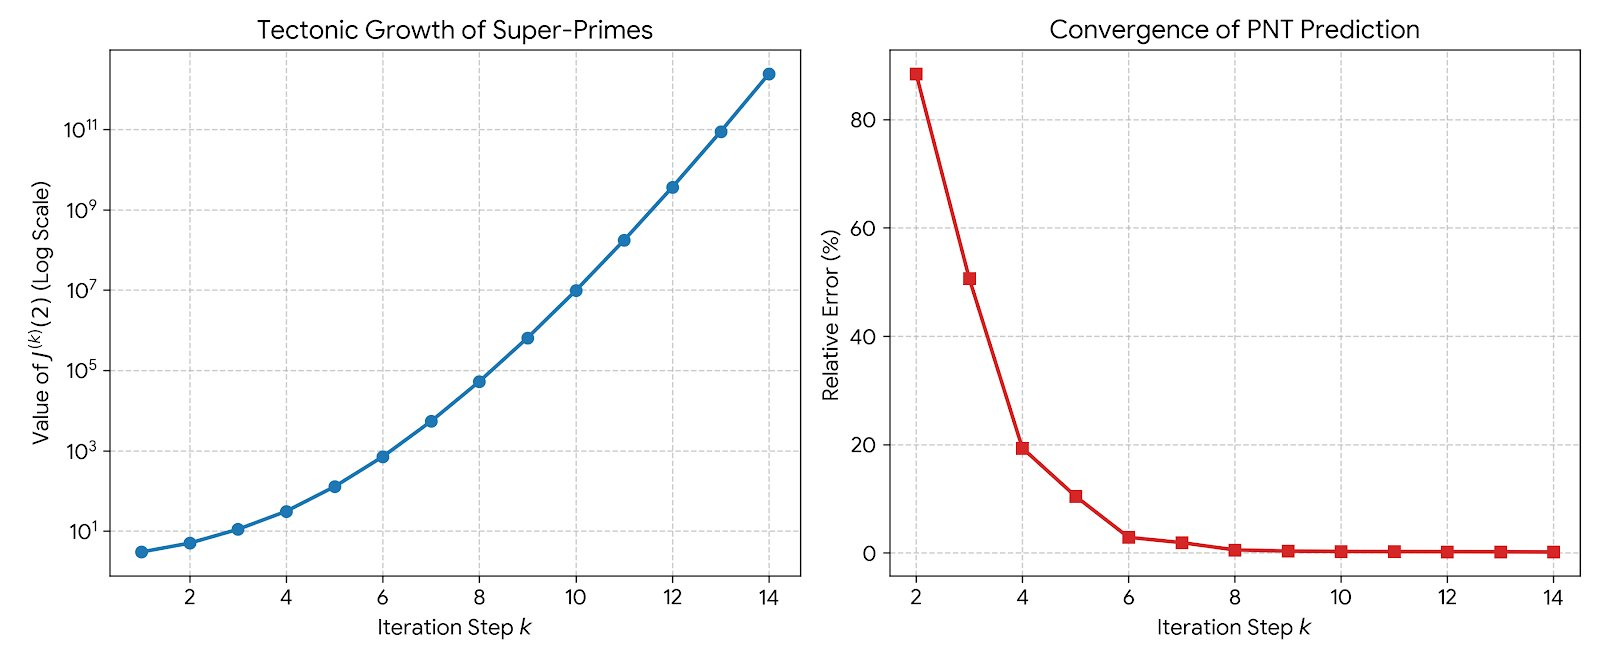
\includegraphics[width=\textwidth]{folding_dynamics.png}
    \caption{\textbf{Left:} Super-polynomial growth of $J^{(k)}(2)$ on a logarithmic scale, showing all 14 iterations. \textbf{Right:} Monotonic convergence of the relative error between empirical data and prediction~\eqref{eq:local_pred}. Only data points for $k \ge 4$ participate in the convergence analysis; the points for $k \le 3$ (where relative errors exceed $50\%$) are displayed in the plot for completeness but fall outside the asymptotic regime, thus their predictions are omitted in Table~\ref{tab:asymptotic_error}.}
    \label{fig:folding_dynamics}
\end{figure}

At iteration $k=14$, the index reached the $10^{11}$ magnitude, requiring $284.6$ seconds. The transition from $k=13$ ($1.22\,$s) to $k=14$ ($284.6\,$s) reflects a roughly $24\times$ increase in the index driving a roughly $233\times$ increase in wall-clock time. While the theoretical time complexity of the pure Meissel--Lehmer algorithm for evaluating $\pi(x)$ is intrinsically sub-linear ($O(x^{2/3}/\ln x)$) \cite{lagarias}, the observed super-linear performance degradation in our empirical data is attributable to implementation artifacts within the computing environment. At the $10^{11}$ magnitude, the execution is dominated by SymPy's memory allocation limits, Python's interpreter overhead, and potential algorithmic fallbacks to sieve-based generation methods, which collectively eclipse the theoretical asymptotic efficiency of the analytic combinatorial algorithm.

\subsection{Computational Limits of Iterated Folding}
Computing $J^{(k)}(2)$ beyond $k = 15$ transitions the requirement from single-node execution to distributed supercomputing. To explore regions at the 100-digit scale ($10^{100}$), exact evaluation of $\pi(x)$ exceeds the capability of all known algorithms on any existing hardware. Methodologies would need to shift to locating \textit{probabilistic super-primes} using randomized primality tests (e.g., Miller--Rabin) over approximated index intervals, though such results cannot be certified as exact.

\section{Conclusion and Future Work}
The PIIA framework unifies principles of abstract algebra with computational number theory, revealing that super-primes are not merely a subsequence of curiosity, but the irreducible atoms of a prime-isomorphic space. The Fundamental Theorem of PIIA (Theorem~\ref{thm:fta}) provides a unique $\otimes$-factorization for every prime, mirroring the classical Fundamental Theorem of Arithmetic. The rigorous asymptotic expansion of the folding operator (Theorem~\ref{thm:asymp}), validated empirically across 14 iterations, demonstrates that the iterated self-reference $J^{(k)}(2)$ is asymptotically well-characterized by nested applications of the Prime Number Theorem.

We emphasize that, as noted in Remark~\ref{rem:transport}, the algebraic isomorphism $f$ ensures that any statement provable in $(\mathbb{P}, \oplus, \otimes)$ is equally provable in $(\mathbb{Z}^+, +, \times)$, and vice versa. The PIIA framework therefore does not provide additional logical power. Its value is heuristic and structural: by studying the metric distortion between the index space and the Euclidean space, classical problems may be viewed from a complementary geometric perspective.

As a concrete example, the Goldbach Conjecture translates into the PIIA domain as a statement about $\oplus$-decomposition into atoms: for every prime with an even index $p_{2k}$ (with $k \ge 2$), there exist two $\otimes$-irreducible elements $q_a, q_b \in \mathbb{P}$ such that $q_a \oplus q_b = p_{2k}$. In the standard integer formulation, the identity $a + b = 2k$ is constrained by the strict requirement that the summands $a$ and $b$ must be prime. Under the PIIA encoding, this constraint on the indices ($a, b \in \mathbb{P}$) maps precisely to the requirement that the PIIA operands $q_a$ and $q_b$ must be super-primes, as established in Theorem~\ref{thm:superp}. This accurately reframes Goldbach's additive decomposition as a fundamental question about the $\oplus$-representability of even-indexed primes strictly by pairs of $\otimes$-irreducible elements, connecting the conjecture directly to the algebraic density results of Corollary~\ref{cor:density}.

Further open problems include: the precise distribution of $\otimes$-irreducible elements in short intervals, the potential further refinement of the error term in Theorem~\ref{thm:asymp} beyond $O(n \ln \ln n)$ (e.g., to an explicit next-order term involving $n$), and the behavior of iterated folding $J^{(k)}$ beyond the current computational frontier.

\vspace{0.5cm}
\noindent \textbf{Code Availability:} The source code for the \textit{Prime-Universe OS} is available at \url{https://github.com/Ruqing1963/Prime-Universe-OS}.

\begin{thebibliography}{99}
\bibitem{broughan} Broughan, K. A., \& Barnett, A. R. (2009). On the Subsequence of Primes Having Prime Indices. \textit{Journal of Integer Sequences}, 12(2), Article 09.2.3.
\bibitem{dusart} Dusart, P. (2010). Estimates of Some Functions Over Primes without R.H. \textit{arXiv preprint arXiv:1002.0442}.
\bibitem{fernandez} Fernandez, N. (1999). An order of primeness, $F(p)$. \textit{Journal of Integer Sequences}, 2(2), Article 99.1.4.
\bibitem{golan} Golan, J. S. (1999). \textit{Semirings and their Applications}. Kluwer Academic Publishers.
\bibitem{hardy} Hardy, G. H., \& Wright, E. M. (2008). \textit{An Introduction to the Theory of Numbers} (6th ed.). Oxford University Press.
\bibitem{lagarias} Lagarias, J. C., Miller, V. S., \& Odlyzko, A. M. (1985). Computing $\pi(x)$: The Meissel--Lehmer method. \textit{Mathematics of Computation}, 44(170), 537--560.
\bibitem{lang} Lang, S. (2002). \textit{Algebra} (Revised Third Edition). Springer-Verlag.
\bibitem{oeis} Sloane, N. J. A. (Ed.). \textit{The On-Line Encyclopedia of Integer Sequences}. Sequence A006450. \url{https://oeis.org}.
\bibitem{rosser} Rosser, J. B., \& Schoenfeld, L. (1962). Approximate formulas for some functions of prime numbers. \textit{Illinois Journal of Mathematics}, 6(1), 64--94.
\end{thebibliography}

\end{document}
